\begin{figure}[H]
  \centering
  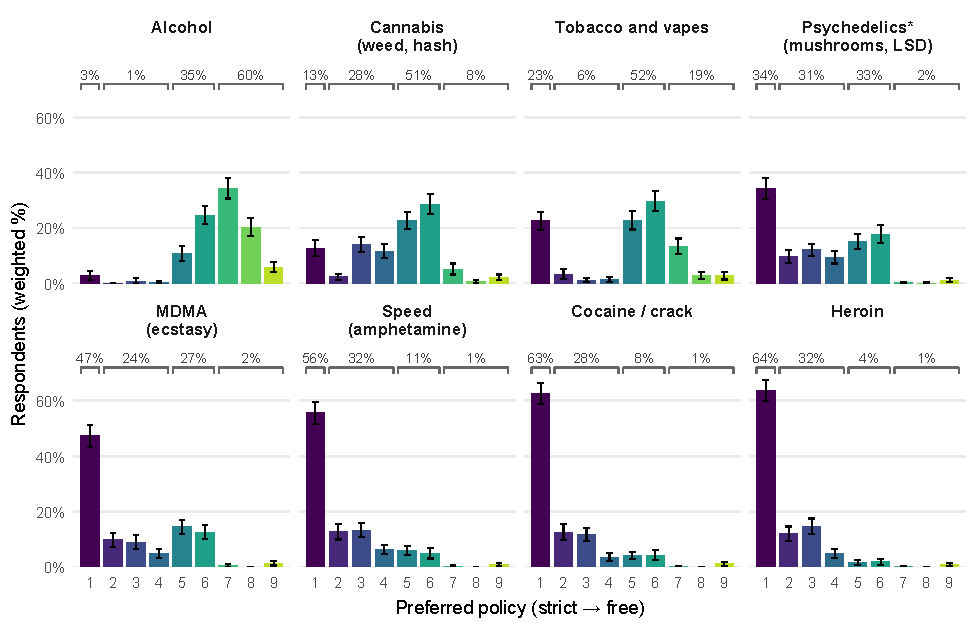
\includegraphics[width=\linewidth]{out/policy_preferences_all_drugs.pdf}
  \caption{Preferred regulatory model per substance. Question: ``Which policy do you think is best?'' (\emph{Welk beleid vindt u het beste?}), with nine options from ban (1) to free sale (9); colours and numbers as in Figure~\ref{fig:policy_scale}. Bars show weighted shares with 95\% confidence intervals; ``no opinion'' is excluded ($n = 1225$--$1234$ per substance). Percentages above the brackets give the weighted share per grouped regime: ban (1), medical/research (2--4), specialist shop (5--6) and general market (7--9). *The item named magic mushrooms and LSD, which are banned in the Netherlands, while psilocybin truffles are legally sold in smartshops; respondents may have had different substances in mind. Panels are ordered by the share choosing a ban. Data: Kieskompas VIP panel, 13--22 October 2026, $n = 1239$, weighted by iterative post-stratification to CBS margins (age, sex, education, migration background, region) and the 2025 Tweede Kamer vote; weights trimmed at the 99th percentile.}
  \label{fig:policy_preferences}
\end{figure}
